\documentclass{jlreq}

\usepackage{amsmath}
\usepackage{array}
\usepackage{bm}
\usepackage{caption}
\usepackage{fancyhdr}
\usepackage{float}
\usepackage{graphicx}
\usepackage{listings}
\usepackage{multirow}
\usepackage{physics}
\usepackage{siunitx}
\usepackage{xcolor}

\lstset{
    language=Verilog, % 使用するプログラム言語を指定
    basicstyle=\ttfamily\footnotesize, % フォントの指定
    tabsize=4, % インデント幅
    numbers=left, % 行番号を表示(必要な場合)
    numberstyle=\tiny, % 行番号のスタイル
    frame=single, % ソースコードを枠で囲む(必要な場合)
    breaklines=true, % 長い行を自動的に折り返す
    captionpos=t, % キャプションの位置を上にする
    showstringspaces=false, % 文字列内のスペースを表示しない
    keywordstyle=\color{blue}, % キーワードの色
    commentstyle=\color{green}, % コメントの色
    stringstyle=\color{red}, % 文字列の色
}
\renewcommand{\lstlistingname}{ソースコード}

\numberwithin{equation}{section}

\pagestyle{fancy}
\fancyhf{}
\fancyhead[R]{\thepage}

\begin{document}

\tableofcontents
\clearpage

\section{実習の目的}
これまでの実習で学んだ事項の総まとめとして,単純な8ビットプロセッサをHDLを用いて設計する.

\section{実験器具}
実験に用いた環境を以下に示す.
\begin{description}
	\item[PC] Inspiron 15 3535
	\item[OS] Windows11
	\item[CPU] AMD Ryzen 5 7530U with Radeon Graphics 2.00 GHz
	\item[統合開発環境] Quartus Prime Lite Edition Version 20.1.1
	\item[FPGAボード] Terasic DE1SoC
\end{description}

\section{理論}
\subsection{アーキテクチャ}
本実習で作成するプロセッサの仕様を表\ref{tab:processor_spec}に示す.
\begin{table}[H]
	\centering
	\caption{作成するプロセッサの仕様}
	\begin{tabular}{c|c}
		\hline
		内部バス幅     & 8ビット \\
		命令数         & 4       \\
		汎用レジスタ数 & 4       \\ \hline
	\end{tabular}
	\label{tab:processor_spec}
\end{table}
このプロセッサは,8ビットの汎用レジスタを4個(R0~R3)備えている.DIN(Data IN)から入力されたデータは,
8ビット幅のマルチプレクサを経由して,これらのレジスタに取り込まれる.

簡略化したブロック図を図\ref{fig:processor_block}に示す.
\begin{figure}[H]
	\centering
	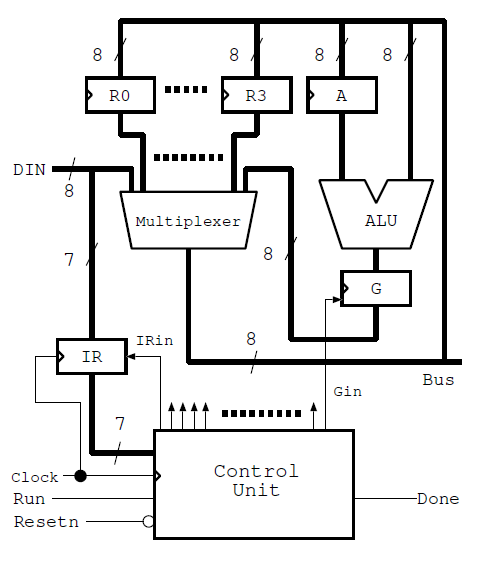
\includegraphics{assets/processor_block_image.png}
	\caption{プロセッサのブロック図}
	\label{fig:processor_block}
\end{figure}
図\ref{fig:processor_block}では,制御ユニットから各構成要素への信号線は一部を除いて省略している.
このプロセッサは,非同期入力Runが1になるとDINから命令を入力し,実行を開始する.命令の実行が完了した時点でDone信号を1にする.
以下,この繰り返しで命令列を実行する.また,非同期リセット入力Resetnを0にすることで,プロセッサ内部の状態を初期化する.

\subsection{プロセッサの設計}
本プロセッサでは,表\ref{tab:instruction_set}に示す4種類の命令を扱う.
表\ref{tab:instruction_set}のRxとRyは,レジスタR0からレジスタR3までのいずれかを指すものとする.また,Dは8ビットの即値を示している.
DIN入力の下位7ビットは命令レジスタ(IR)に接続し,制御ユニットが入力制御信号$IR_{in}$を1にしたときに,命令コードをIRから取り込む.
\begin{table}[H]
	\centering
	\caption{命令セット}
	\begin{tabular}{c|l|l}
		\hline
		命令コード & 命令              & 動作                        \\ \hline
		000        & mv Rx, Ry         & Rx $\leftarrow $[Ry]        \\
		001        & mvi Rx, $\sharp$D & Rx$\leftarrow$D             \\
		010        & add Rx, Ry        & Rx $\leftarrow$ [Rx] + [Ry] \\
		011        & sub Rx, Ry        & Rx$\leftarrow$[Rx]-[Ry]     \\ \hline
	\end{tabular}
	\label{tab:instruction_set}
\end{table}

このプロセッサの命令構成を図\ref{fig:instruction_composition}に示す.
\begin{figure}[H]
	\centering
	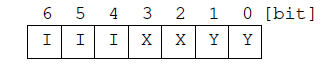
\includegraphics{assets/instruction_composition.png}
	\caption{命令構成}
	\label{fig:instruction_composition}
\end{figure}

\subsubsection{レジスタ部の設計}
プロセッサではDINから入力した命令コードに従って,データを汎用レジスタとAレジスタ間で移動させ,ALUで演算を行う.
そのためにはマルチプレクサの出力を適切に選択しなければならない.マルチプレクサと汎用レジスタの接続図を図\ref{fig:mux_to_register}に示す.
図\ref{fig:mux_to_register}のように,4個の汎用レジスタ(R0~R3)と入力DINをマルチプレクサに接続し,選択信号Sで指定したレジスタまたはDINの値をMUXから出力させる.
MUXからの出力は各レジスタの入力に接続し,入力制御信号が1になっているレジスタにのみ入力できるようにする.
また,各レジスタにはリセット信号を接続し,リセット入力によりレジスタの内容がゼロクリアできるようにする.
\begin{figure}[H]
	\centering
	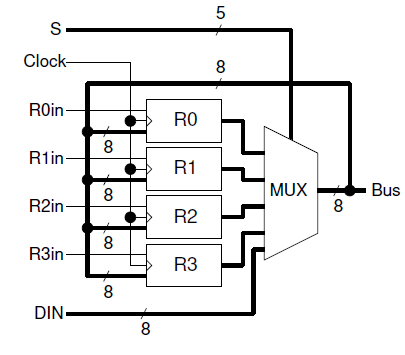
\includegraphics{assets/mux_to_register.png}
	\caption{マルチプレクサからレジスタへの入力}
	\label{fig:mux_to_register}
\end{figure}

\subsubsection{ALU部の設計}
一般的なALUでは論理演算,算術演算,シフト演算の機能を持つが,本実習では基本的な算術演算(加減算)だけを行うものとする.
演算の種類を選択するための制御信号(演算選択信号)は,扱う演算が加減算の2種類しかないため,1ビット幅で良い.
この演算選択信号を,ALUモジュールへの入力として接続する.
Aレジスタと汎用レジスタを用いてALUで演算を行い,結果をGレジスタに格納する.

\subsubsection{制御ユニットの設計}
制御ユニットは,DINからIRに入力した命令を解釈し,どのタイミングで値をレジスタに取り込むか,またマルチプレクサではどの入力を選択するかといった制御を行う.
これらの操作は,命令が定まった時点で一意に決まり,組み合わせ回路で構成することができる.しかし,即値を取り込む場合など,命令によっては実行完了までに数サイクルを要するものがある.
そこで,制御ユニットの内部ではタイムステップを管理する有限状態機械を構成し,各ステップでの動作を定めるものとする.
このように,制御ユニットは有限状態機械と組み合わせ回路を組み合わせて構成することができる.

\section{演習の解答}
\subsection{演習1}
内部構成について先に触れる.マルチプレクサで入力信号の数を6個から16個に増やす必要性が生じると考えられる.
また,制御ユニットにて選択信号を

\subsection{演習2}

\section{実習}
\subsection{実習1}
図\ref{fig:mux_to_register}のような回路をVerilog HDLで記述したモジュールをソースコード\ref{src:register_mux_part}に示す.
\begin{lstlisting}[caption={実習1のモジュール}, label={src:register_mux_part}]
module jisshu1(Clk, Resetn, DIN, S, R0in, R1in, R2in, R3in, Bus);
	input Clk, Resetn, R0in, R1in, R2in, R3in;
	input [4:0] S;
	input [7:0] DIN;
	output [7:0] Bus;
	wire [7:0] Bus, R0out, R1out, R2out, R3out;
	
	register R0(Clk, Resetn, Bus, R0in, R0out);
	register R1(Clk, Resetn, Bus, R1in, R1out);
	register R2(Clk, Resetn, Bus, R2in, R2out);
	register R3(Clk, Resetn, Bus, R3in, R3out);
	
	mux MUX(S, R0out, R1out, R2out, R3out, DIN, Bus);
endmodule

module register(Clk, Resetn, D, EN, Q);
	input Clk, Resetn, EN;
	input [7:0] D;
	output reg [7:0] Q;
	
	always @(posedge Clk or negedge Resetn) begin
		if(!Resetn)
			Q <= 0;
		else if(EN)
			Q <= D;
	end
endmodule

module mux(S, R0, R1, R2, R3, DIN, Bus);
	input [4:0] S;
	input [7:0] R0, R1, R2, R3, DIN;
	output wire [7:0] Bus;
	
	assign Bus = (S == 6'b000001) ? R0 : (
					 (S == 6'b000010) ? R1 : (
					 (S == 6'b000100) ? R2 : (
					 (S == 6'b001000) ? R3 : (
					 (S == 6'b010000) ? DIN : 6'bxxxxxx))));
endmodule
\end{lstlisting}

このモジュールが正しく動くかどうかをシミュレーションにより確認する.
ソースコード\ref{src:register_mux_part}をRTL Viewerで出力したものを図\ref{fig:jisshu1_RTL}に,シミュレーション結果を図に示す.
図\ref{fig:jisshu1_sim}のシミュレーション結果では,DINから様々な値をレジスタに入力している.
また,レジスタ間でデータの移動を行っており,EN信号が与えられらレジスタのみ入力されていることが分かる.
最終的に全レジスタが同じ値を持っており,コード\ref{src:register_mux_part}が正しく動いていることが確認できた.
\begin{figure}[H]
	\centering
	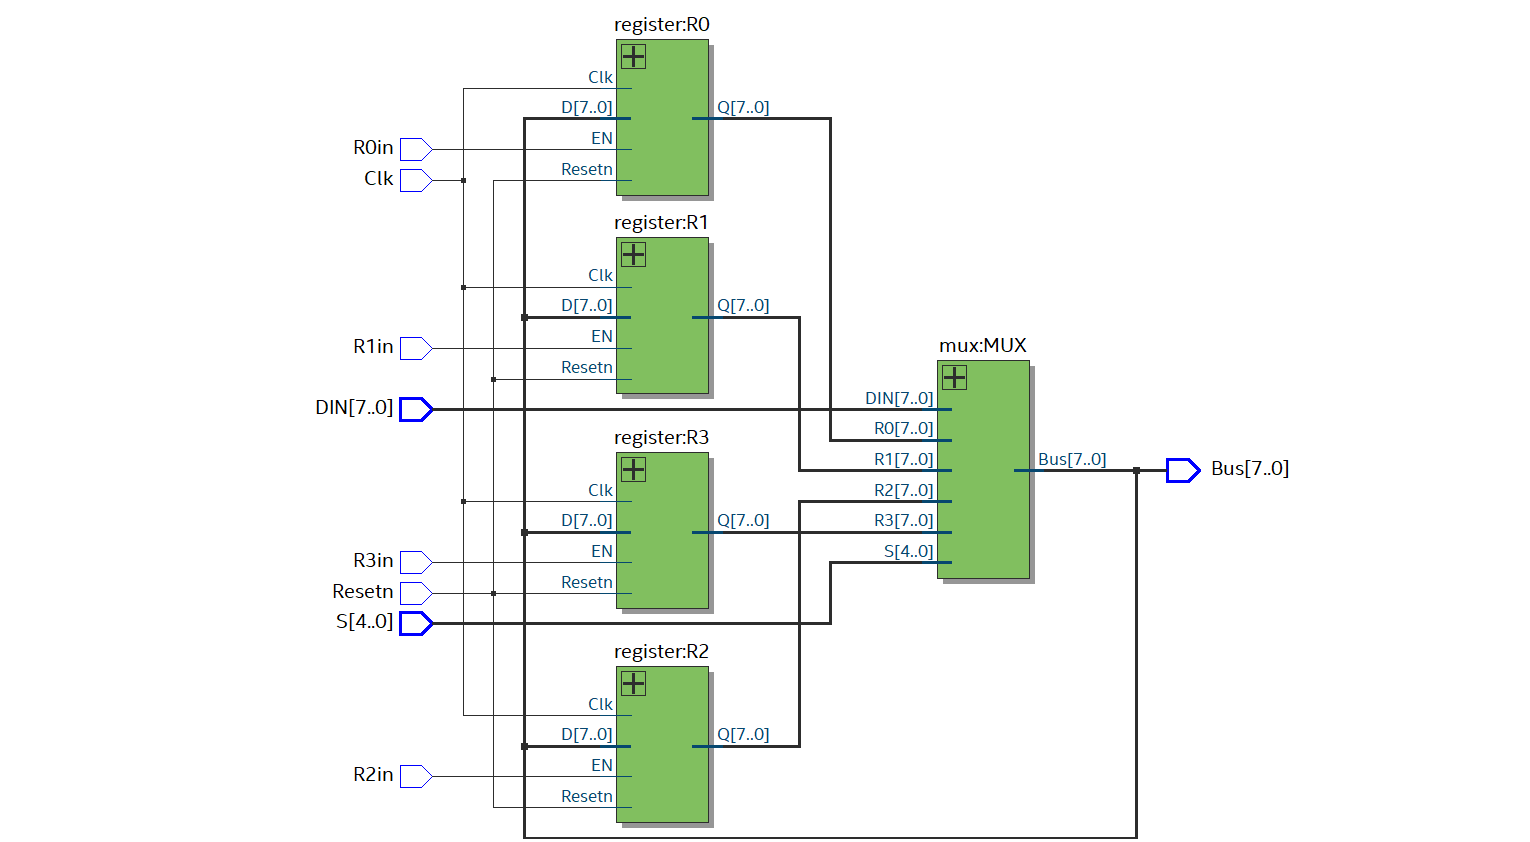
\includegraphics[width=\textwidth]{assets/jisshu1_RTL.png}
	\caption{ソースコード\ref{src:register_mux_part}からRTL Viewerで出力した回路図}
	\label{fig:jisshu1_RTL}
\end{figure}

\begin{figure}[H]
	\centering
	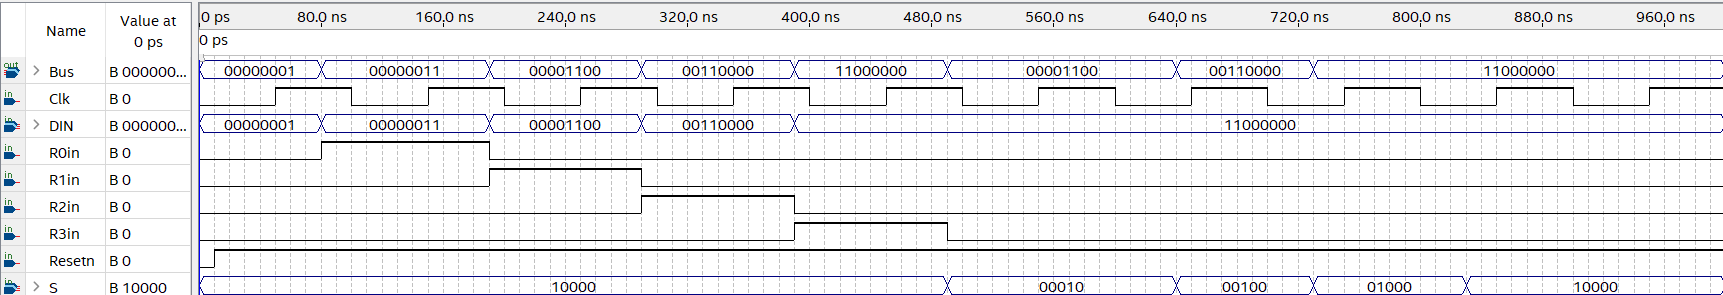
\includegraphics[width=\textwidth]{assets/jisshu1_sim.png}
	\caption{ソースコード\ref{src:register_mux_part}のシミュレーション結果}
	\label{fig:jisshu1_sim}
\end{figure}

\subsection{実習2}
ALUモジュールとAレジスタおよびGレジスタをVerilog HDLで記述し,実習1で作成した回路に追加したものを
ソースコード\ref{src:jisshu2}に示す.
\begin{lstlisting}[caption={実習2のモジュール}, label={src:jisshu2}]
module jisshu2(Clk, Resetn, DIN, S, R0in, R1in, R2in, R3in, Ain, Gin, Mode, OF, R0out, R1out, R2out, R3out, Aout, Gout, Bus);
	input Clk, Resetn, R0in, R1in, R2in, R3in, Ain, Gin, Mode;
	input [5:0] S;
	input [7:0] DIN;
	output wire [7:0] Bus, R0out, R1out, R2out, R3out, Aout, Gout;
	output OF;
	wire [7:0] ALUout;
	wire of;
	
	register R0(Clk, Resetn, Bus, R0in, R0out);
	register R1(Clk, Resetn, Bus, R1in, R1out);
	register R2(Clk, Resetn, Bus, R2in, R2out);
	register R3(Clk, Resetn, Bus, R3in, R3out);
	mux MUX(S, R0out, R1out, R2out, R3out, DIN, Gout, Bus);
	
	ALU ALU(Aout, Bus, Mode, of, ALUout);
	register A(Clk, Resetn, Bus, Ain, Aout);
	register G(Clk, Resetn, ALUout, Gin, Gout);
	D_FF OF_DFF(Clk, Resetn, of, OF);
endmodule

module register(Clk, Resetn, D, EN, Q);
	input Clk, Resetn, EN;
	input [7:0] D;
	output reg [7:0] Q;
	
	always @(posedge Clk or negedge Resetn) begin
		if(!Resetn)
			Q <= 0;
		else if(EN)
			Q <= D;
	end
endmodule

module mux(S, R0, R1, R2, R3, DIN, Gout, Bus);
	input [5:0] S;
	input [7:0] R0, R1, R2, R3, DIN, Gout;
	output wire [7:0] Bus;
	
	assign Bus = (S == 6'b000001) ? R0 : (
					 (S == 6'b000010) ? R1 : (
					 (S == 6'b000100) ? R2 : (
					 (S == 6'b001000) ? R3 : (
					 (S == 6'b010000) ? DIN : (
					 (S == 6'b100000) ? Gout: 6'bxxxxxx)))));
endmodule

module ALU(A, B, MODE, OF, S);
	input [7:0] A, B;
	input MODE;
	output [7:0] S;
	output OF;
	
	wire [7:0] A_comp;
	wire c1, c2, c3, c4, c5, c6, c7, cout;
	
	assign A_comp = (MODE) ? ~A : A;
	
	FA FA_0(A_comp[0], B[0], MODE, S[0], c1);
	FA FA_1(A_comp[1], B[1], c1, S[1], c2);
	FA FA_2(A_comp[2], B[2], c2, S[2], c3);
	FA FA_3(A_comp[3], B[3], c3, S[3], c4);
	FA FA_4(A_comp[4], B[4], c4, S[4], c5);
	FA FA_5(A_comp[5], B[5], c5, S[5], c6);
	FA FA_6(A_comp[6], B[6], c6, S[6], c7);
	FA FA_7(A_comp[7], B[7], c7, S[7], cout);
	
	assign OF = (A_comp[7] == B[7]) && (S[7] != B[7]);
endmodule

module FA(A, B, Cin, S, Cout);
	input A, B, Cin;
	output S, Cout;
	
	assign S = (A ^ B) ^ Cin;
	assign Cout = (A ^ B) & Cin | A & B;
endmodule

module D_FF(Clk, Resetn, D, Q);
	parameter bitwidth = 1;
	
	input Clk, Resetn;
	input [bitwidth-1:0] D;
	output reg [bitwidth-1:0] Q;
	
	always @(posedge Clk or negedge Resetn) begin
		if(!Resetn)
			Q <= 0;
		else
			Q <= D;
	end
endmodule
\end{lstlisting}

ALU部が正しい挙動をするかどうかをシミュレーションで確認した.ソースコード\ref{src:jisshu2}からRTL Viewerで出力した回路図を図\ref{fig:jisshu2_RTL}に,シミュレーション結果を図\ref{fig:jisshu2_sim}に示す.
\begin{figure}[H]
	\centering
	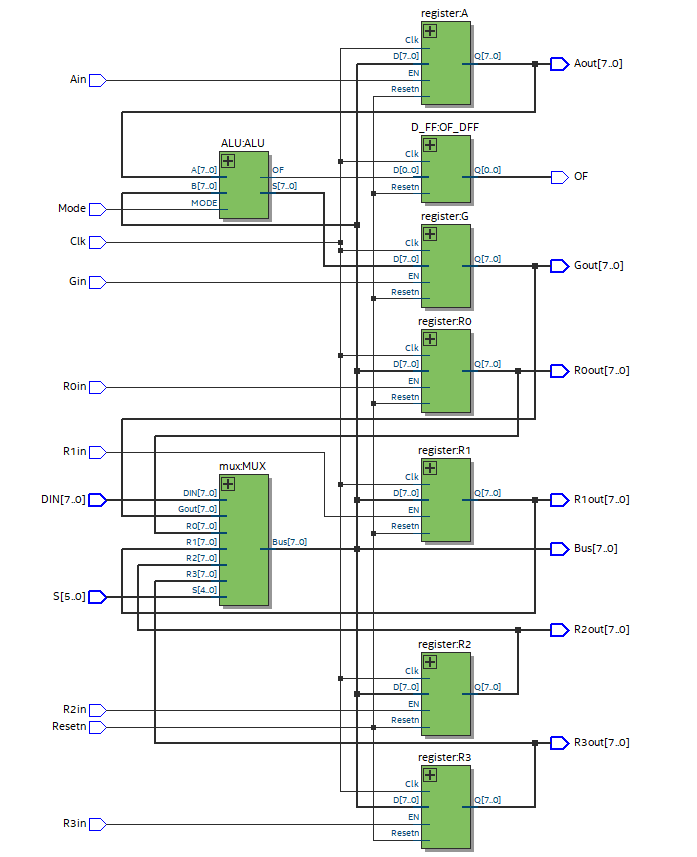
\includegraphics[width=\textwidth]{assets/jisshu2_RTL.png}
	\caption{ソースコード\ref{src:jisshu2}からRTL Viewerで出力した回路図}
	\label{fig:jisshu2_RTL}
\end{figure}

\begin{figure}[H]
	\centering
	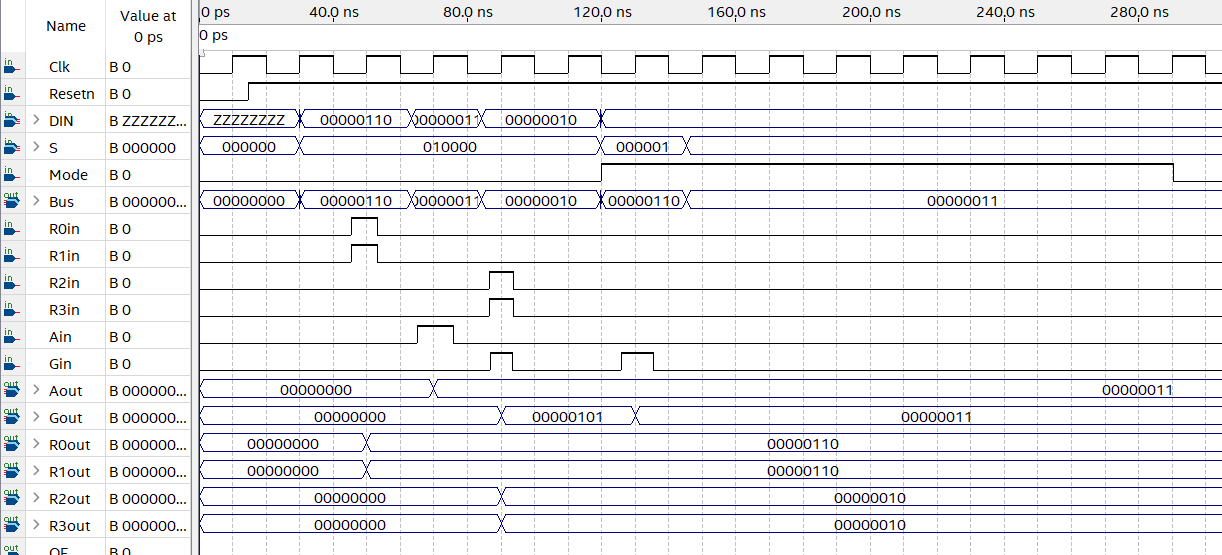
\includegraphics[width=\textwidth]{assets/jisshu2_sim.png}
	\caption{実習2のシミュレーション結果}
	\label{fig:jisshu2_sim}
\end{figure}

Mode = 0の加算の場合から確認する.$70[\si{\ns}]$でAレジスタに$(00000011)_{2}$を入力している.
そして,$90[\si{\ns}]$でGレジスタの入力制御信号を1にしてGレジスタに演算結果を格納している.このとき,Busを流れているのは$(00000010)_2$なので演算結果は
$(00000011)_{2} + (00000010)_2 = (00000101)_2$になるはずである.Goutの値を見ると,きちんと反映されている.よって,加算に関しては正しく動いたことが確認できた.

次に,$120[\si{\ns}]$でMode = 1とした.そして,選択信号をDINではなく汎用レジスタ(R0)に指定した.R0には$(00000110)_2$が格納されており,$130[\si{\ns}]$でGレジスタの制御信号を1にしたときは$A_{out}$には$(00000011)_2$が格納されている.
したがって,演算結果は$(00000110)_2 - (00000011)_2 = (00000011)_2$となるはずである.Goutの値を確認すると,きちんと反映されており,減算についても正しい動作をしていることが確認できた.
以上から,ALU部分の実装は正しくできた.

\subsection{実習3}

\section{考察}

\begin{thebibliography}{9}
	\bibitem{exp_text} 布目 淳.プロジェクト実習Ⅲ 論理設計 実験テキスト.京都工芸繊維大学,2024年
	\bibitem{user_manual} Terasic Technologics Inc.:  ``DE1-SoC User Manual V2.0.4'' Chapter3. Using the DE1-SoC Board, 2019
\end{thebibliography}

\end{document}